%; whizzy section -pdf xpdf -latex ./whizzypdfptex.sh
% latex beamer presentation.
% platex, latex-beamer でコンパイルすることを想定。 

%     Tokyo Debian Meeting resources
%     Copyright (C) 2008 Junichi Uekawa

%     This program is free software; you can redistribute it and/or modify
%     it under the terms of the GNU General Public License as published by
%     the Free Software Foundation; either version 2 of the License, or
%     (at your option) any later version.

%     This program is distributed in the hope that it will be useful,
%     but WITHOUT ANY WARRANTY; without even the implied warranty of
%     MERCHANTABILITY or FITNESS FOR A PARTICULAR PURPOSE.  See the
%     GNU General Public License for more details.

%     You should have received a copy of the GNU General Public License
%     along with this program; if not, write to the Free Software
%     Foundation, Inc., 51 Franklin St, Fifth Floor, Boston, MA  02110-1301 USA

\documentclass[cjk,dvipdfmx,12pt]{beamer}
\usetheme{Tokyo}
\usepackage{monthlypresentation}

%  preview (shell-command (concat "evince " (replace-regexp-in-string "tex$" "pdf"(buffer-file-name)) "&"))
%  presentation (shell-command (concat "xpdf -fullscreen " (replace-regexp-in-string "tex$" "pdf"(buffer-file-name)) "&"))

%http://www.naney.org/diki/dk/hyperref.html
%日本語EUC系環境の時
\AtBeginDvi{\special{pdf:tounicode EUC-UCS2}}
%シフトJIS系環境の時
%\AtBeginDvi{\special{pdf:tounicode 90ms-RKSJ-UCS2}}

\title{東京エリア Debian 勉強会}
\subtitle{資料}
\author{上川 純一 dancer@debian.org\\IRC nick: dancerj}
\date{2008年5月17日}
\logo{
\includegraphics[width=8cm]{image200607/openlogo-light.eps}}

\begin{document}

\frame{\titlepage{}}


\section{Intro}

\emtext{設営準備にご協力ください}

\begin{frame}
 \frametitle{Agenda}
\begin{minipage}[t]{0.45\hsize}
  \begin{itemize}
  \item 注意事項
	\begin{itemize}
	 \item 飲食禁止
	 \item 政治/宗教/営利活動禁止
	\end{itemize}
  \item quiz
  \item 最近のDebian関連のイベント
	\begin{itemize}
	 \item 前回 
	 \item eeePC Open Source Developer's Conference 
	\end{itemize}
 \end{itemize}
\end{minipage} 
\begin{minipage}[t]{0.45\hsize}
 \begin{itemize}
  \item バイナリをわけたパッケージの扱い
  \item OpenSSL セキュリティーホール速報
  \item kFreeBSD / Nexenta / Hurd / SuperH
 \end{itemize}
\end{minipage}
\end{frame}

\section{最近}


\begin{frame}
 \frametitle{前回のAgenda}
\begin{minipage}[t]{0.45\hsize}
  \begin{itemize}
  \item 注意事項
	\begin{itemize}
	 \item 飲食禁止
	 \item 政治/宗教/営利活動禁止
	\end{itemize}
  \item quiz
  \item 最近のDebian関連のイベント
	\begin{itemize}
	 \item 前回 
	\end{itemize}
 \end{itemize}
\end{minipage} 
\begin{minipage}[t]{0.45\hsize}
 \begin{itemize}
  \item バイナリ一つだけのパッケージを作成してみる
  \item バージョン管理ツールを使い Debian パッケージを管理する Git編
  \item アップストリームの VCS と付き合う
  \item Nexenta Core Platformを使ってみる
 \end{itemize}
\end{minipage}
\end{frame}

\begin{frame}{eeePC Open Source Developer's Conference 1/2}
\begin{minipage}[t]{0.45\hsize}
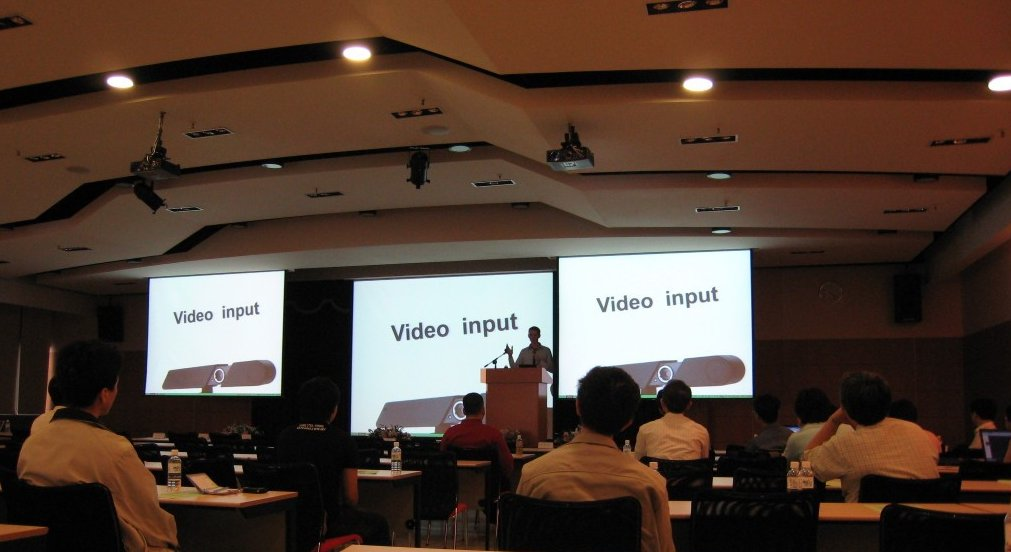
\includegraphics[width=0.9\hsize]{image200805/eeepcdevconf-place.jpg}

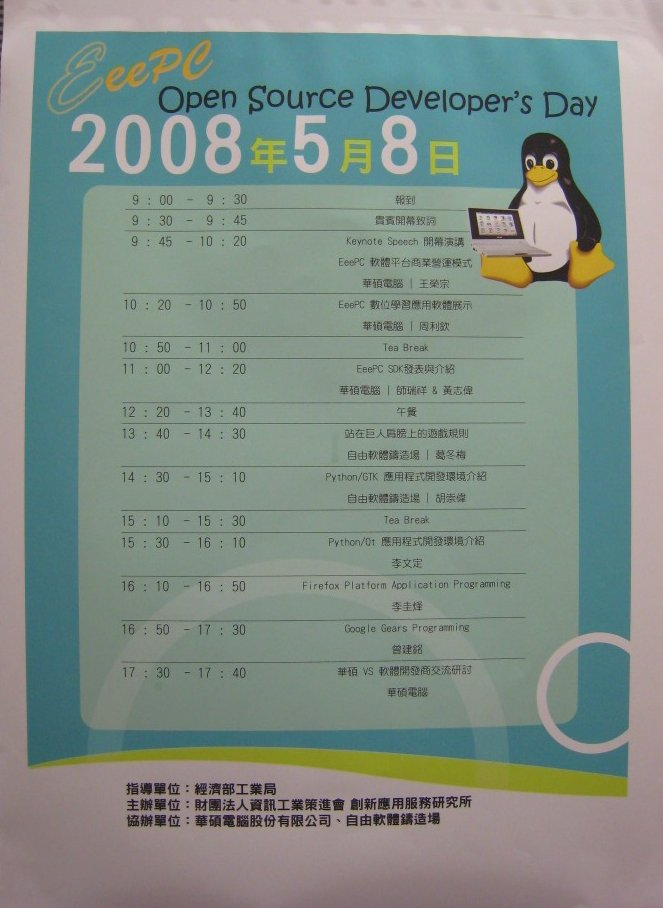
\includegraphics[width=0.45\hsize]{image200805/eeepcdevconf-agenda1.jpg}
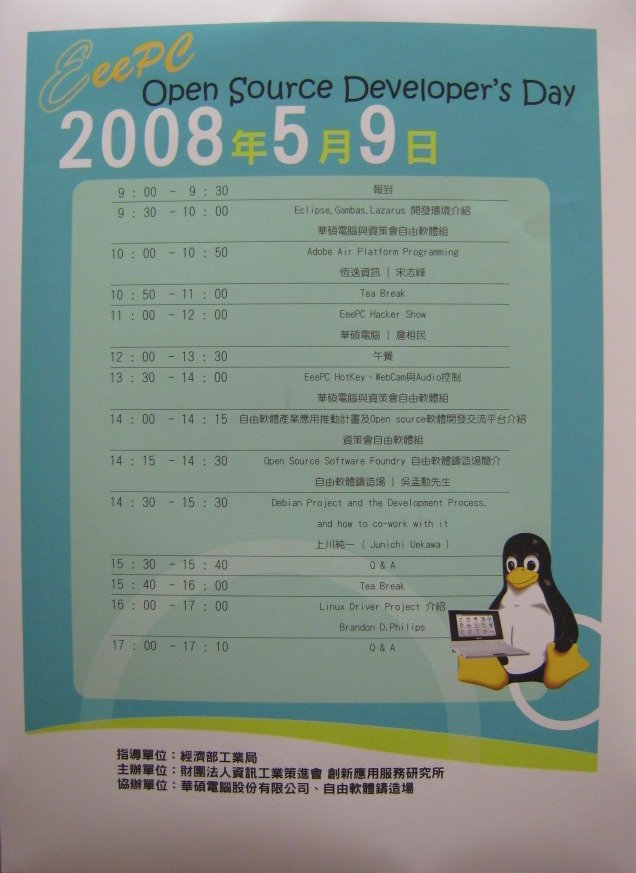
\includegraphics[width=0.45\hsize]{image200805/eeepcdevconf-agenda2.jpg}

\end{minipage}
\begin{minipage}[t]{0.45\hsize}
\begin{itemize}
 \item 台北市内
 \item 100人程度の参加
 \item eeePC を冠にしたオープンソース開発者のためのカンファレンス
 \item 5月8日・9日
\end{itemize}
\end{minipage}
\end{frame}

\begin{frame}{eeePC Open Source Developer's Conference 2/2}

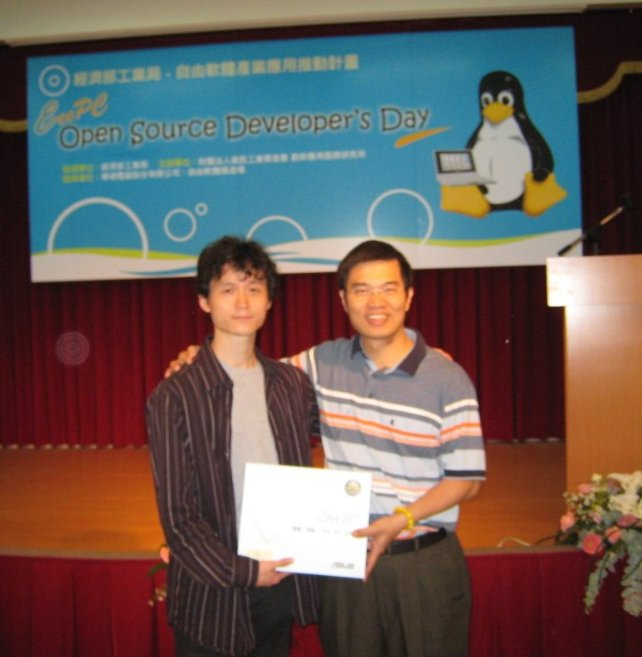
\includegraphics[width=1\hsize]{image200805/eeepc-give.jpg}

\end{frame}

\begin{frame}{夜の街}

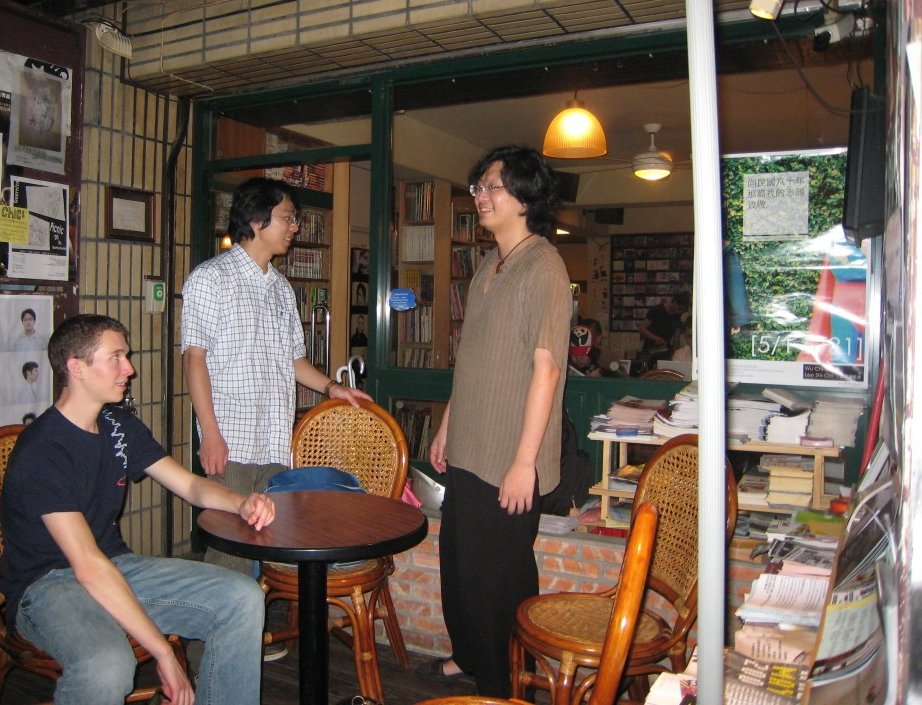
\includegraphics[width=0.45\hsize]{image200805/nightpub1.jpg}
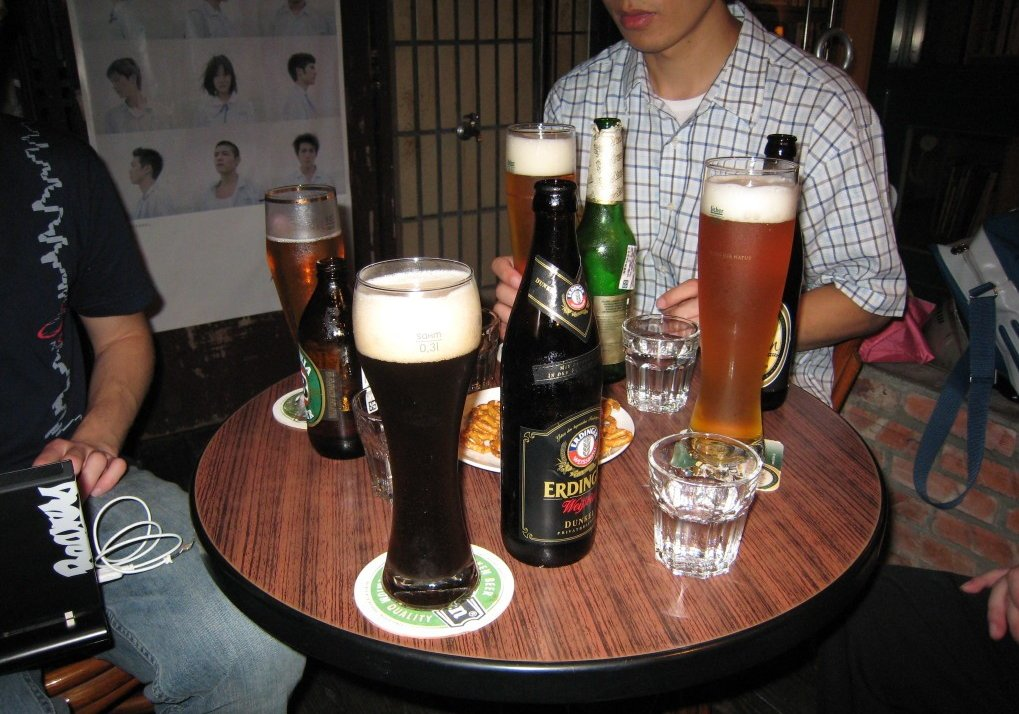
\includegraphics[width=0.45\hsize]{image200805/nightpub2.jpg}

みんなこういうところで毎日ハックしているらしい。

\end{frame}


\begin{frame}{台湾Debian勉強会キックオフ}
\begin{minipage}[t]{0.45\hsize}
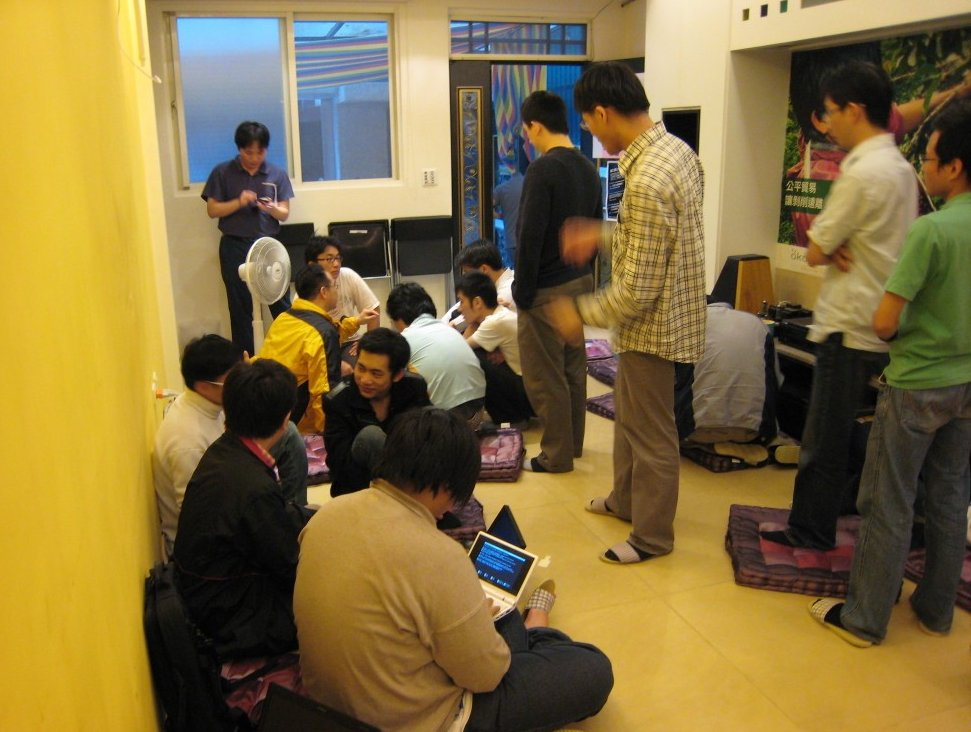
\includegraphics[width=0.9\hsize]{image200805/taipeidebian.jpg}
\end{minipage}
\begin{minipage}[t]{0.45\hsize}
\begin{itemize}
 \item 台北市内のカフェ、無線LAN完備
 \item 20人程度参加
\end{itemize}
\end{minipage}
\end{frame}



\section{DWN quiz}
\begin{frame}{Debian 常識クイズ}

Debian の常識、もちろん知ってますよね?
知らないなんて恥ずかしくて、知らないとは言えないあんなことやこんなこと、
みんなで確認してみましょう。

今回の出題範囲は\url{debian-devel-announce@lists.debian.org} に投稿された
内容とDebian Project Newsからです。

\end{frame}

\subsection{問題}

%問題をコピペ

 \santaku
 {Joerg Jaspertがdakのソースコードに取り込んだ、Thomas Viehmannからのパッチとは?}
 {パッケージを受け取ったときにメンテナだけでなくスポンサーにもメールを送るようにするパッチ}
 {パッケージを受け取ったときに現在のカルマをメンテナに通知するパッチ}
 {パッケージを受け取ったときに現在のバグの一覧をメンテナに通知するパッチ}
 {A}
 
 \santaku
 {debhelperバージョン7では、何から学んだことを取り込んでいるか}
 {MSDN}
 {CDDB}
 {CDBS}
 {C}
 
 \santaku
 {新たにリリースマネージャになったのは?}
 {Andreas Barth}
 {Luk Claes}
 {Marc 'HE' Brockschmidt}
 {C}
 
 \santaku
 {Debianパッケージメンテナンスに関する自動通知メールにおいて、メールを生成したソフトウェアを示すのに使うよう提案されたメールヘッダは?}
 {X-Debian:}
 {X-Debian-Package:}
 {User-Agent:}
 {A}
 
 \santaku
 {Siobh\'an O'MahonyとFabrizio Ferraroの研究ではDebianの統治システムの歴史を4つの時期に分けているが、そのうち1999年から2003年に当たるものは?}
 {Stabilizing Governance}% 2003-2006
 {Implementing Governance}% 1999-2003
 {Designing Governance}% 1997-1999
 {B}
 
 \santaku
 {Institute for Advanced Professional Studies Yankee groupの研究結果として適切でないものは?}
 {2006年と比べてDebianサーバのダウンタイムが41\%{}減った}
 {2006年と比べてネットワークに1台以上のDebianを入れているユーザが15\%{}から24\%{}に上昇した}
 {2006年と比べてDebianユーザが41\%{}減った}
 {C}
 
 \santaku
 {開発者のブログ記事を収集して表示するPlanet Debianに関して、Martin Joey Schulzeが始めたサービスとは?}
 {記事をメーリングリストとして購読できるようにするサービス}
 {すべての記事に対してコメントを一斉に送れるようにするサービス}
 {記事をSlashdotや各種ソーシャルブックマークサービスに容易に投稿できるようにするサービス}
 {A}
 
 \santaku
 {Christian Perrierによると、最近正式なDebian開発者として登録されたメンバーの女性率は?}
 {5\%{}}
 {10\%{}}
 {50\%{}}
 {B}

 \santaku
 {WWWの生みの親として有名なTim Berners-LeeがWWW2008カンファレンスの基調演説でDebianについて述べたこととは?}
 {Debianのウェブページのように古臭いページは消えていく運命にある}
 {Debianのウェブページは様々な言語に地域化されており素晴らしい}
 {Debianのパッケージングシステムは素晴らしい}
 {C}
 
 \santaku
 {今年のGoogle Summer of CodeプログラムでDebian Projectのタスクを得た学生の人数は?}
 {6}
 {12}
 {24}
 {B}
 
 \santaku
 {5月9日現在、lennyのリリースに向けて進められている移行の状況として適切でないものは?}
 {Perlのバージョン5.10をlennyでデフォルトとするための移行作業が行われている}
 {既にlennyにおいてPythonのデフォルトがバージョン2.5になっている}
 {Rubyのバージョン1.9をlennyでデフォルトとするための移行作業が行われている}
 {C}
 
 \santaku
 {4月18日に何人のDebian正式開発者が追加されたか?}
 {9}
 {19}
 {29}
 {B}

\section{事前課題紹介}
\emtext{事前課題の紹介}
% pre work home work

\begin{frame}{事前課題問題}

\begin{enumerate}
 \item 「フリーになって嬉しい/なると嬉しいソフトウェア」
 \item 「パッケージになって嬉しい/なると嬉しい/するのは難しそうなソフ
       トウェア」
 \item 「僕がゴールデンウィークに自由なソフトウェアのために行ったこと」
\end{enumerate}

\end{frame}

% (query-replace "\\subsection" "\\end{frame}\\begin{frame}")
% (query-replace "\\subsubsection" "\\textbf")


\begin{frame}{前田 耕平}

「フリーになって嬉しい/なると嬉しいソフトウェア」

djbdnsです。qmailははっきり言ってどうでも良いのですが、djbdnsは重宝してます。設定が簡単なのと、OpenBlockSでBINDを動かすのは重すぎるので軽快なdjbdnsとdnscacheは無いと困るので、今まではOBS用のコンパイル環境として古いiBookでビルドしてからOBSに流し込んでました。サーバにコンパイラを入れるのはナンセンスなので。

「パッケージになって嬉しい/なると嬉しい/するのは難しそうなソフトウェア」

Hobbit。これもこれでOBS用にビルドしないで済むようになったので。

「僕がゴールデンウィークに自由なソフトウェアのために行ったこと」

GWは子供の日が誕生日の嫁への奉仕が70%、家事が25%、今回の発表用の資料の下書き作成に5%でした。
\end{frame}\begin{frame}{岩松}

「フリーになって嬉しい/なると嬉しいソフトウェア」
\begin{itemize}
 \item   Flash plugin\\
 先日 Flash に関するライセンスの変更がありましたけど、開発が
 少しは楽になるのかな、と思います。
\end{itemize}

「僕がゴールデンウィークに自由なソフトウェアのために行ったこと」

\begin{itemize}
 \item   Macbook iSight のファームウェアハック
 \item  Backlight をコントロールするための Xfce4 プラグインの開発
 \item  Xradnr を設定するための GUI開発 および Xfce4 プラグインの開発
 \item  Xfce の翻訳
 \item  U-boot for SuperH の開発
 \item  Debian kenrel module auto builder の妄想
 \item  Debian/SH の開発
\end{itemize}


\end{frame}\begin{frame}{堀内寛己}

僕は無職の精神病者で、障害年金で暮らしています。
それで、毎日日曜プログラミングをしています。
自由なソフトウェアの作者として、ある意味究極の境遇にあるのかもしれません。

「僕がゴールデンウィークに自由なソフトウェアのために行ったこと」

ですから、ゴールデンウィークだからといって普段と差があるわけではありません。
たまたまこの時期、そして今も取り組んでいるのは、
レスキューOS作成用の、live-helperより気の利いたスクリプトの開発です。

このレスキューOSのファイルシステムは、USBフラッシュかNFSに置き、
必要なとき「だけ」CDに、ブートローダー「だけ」を置きます。

\end{frame}\begin{frame}{堀内寛己}

どうもlive-helperは、こういう用途に向いていないように思います。
live-helperの構成パラメータは山ほどありますが、これは
山ほど構成して1枚に焼きこんで、試してだめなら構成しなおし焼き直し、
という使い方を想定しているからに思えます。
僕が目指しているのはそういうものではありません。

live-helperの開発者は、LiveCD作りの発想から抜け出せないようです。
誤解があったら指摘してください。

\end{frame}\begin{frame}{やまねひでき}

「フリーになって嬉しい/なると嬉しいソフトウェア」

\begin{itemize}
 \item adobe-cmap - これでハマることが多すぎです。
\end{itemize}

「パッケージになって嬉しい/なると嬉しい/するのは難しそうなソフトウェア」
 パッケージにした/しようとして止まっているのとかはあります。

\begin{itemize}
 \item  mirmon	-- ミラーサーバの状態チェックができます。スポンサー待ちで半年以上…
 \item  gnview	-- gtk2-perl の 2ch ブラウザ。スポンサー待ちです。
 \item  FailSafeC  -- 安全なC言語コンパイラ。upstream の man 作成やライセンスの確認待ち
 \item  naist-jdic -- non-free な ipadic の置き換え。upstream の作業待ち。
\end{itemize}

\end{frame}\begin{frame}{やまねひでき}

「僕がゴールデンウィークに自由なソフトウェアのために行ったこと」

ゴールデンウィークって何?だったので…
まぁ、いつも通りにパッケージのアップデートとかでした。
あ、そうそうミラーサーバの復旧作業してきました。機材は Ubuntu Japanese Team の方
から提供いただき、増設HDDは自費購入。

\end{frame}\begin{frame}{吉田@板橋}

僕がゴールデンウィークに自由なソフトウェアのために行ったこと

ゴールデンウィーク(GW)には家のサーバのファイル名等のエンコーディングを
eucJPからUTF-8に変更する作業を行っていました。
そろそろ変えておいた方が、他の環境(今時のディストリービューションや
Windows等)との相互運用性が良いと判断し、時間がとれるGWに作業しました。
基本的にサービスを絞ったサーバ運用だったので、ファイル名変更のほかはsamba
やapache、bash等の設定変更のみでいけました。
その準備(バックアップ)として、漢字ファイル名を使用しているファイルに対
してkakasiおよびハードリンクを使用してローマ字にリネームするスクリプトを
(似たようなことをしているwebの記述を参考に)作成し、適用しました。
そのログやスクリプトはwebにある自分の備忘録に上げておきました、ご参考ま
で。


\end{frame}\begin{frame}[containsverbatim]{あけど}

お題: パッケージになって嬉しい/なると嬉しい/するのは難しそうなソフトウェア

 実は「フリーになって嬉しい/なると嬉しいソフトウェア」ってのがあるのですが
たぶん他の方が触れられるかと思いますので、一つだけ挙げておきます。

\begin{commandline}
 adobe-cmap
\end{commandline}

これって元ネタはRFCらしいのですが、どうなったんでしょう?

\end{frame}\begin{frame}{あけど}

 では本題、パッケージになって嬉しいというか「こんなのあったらなぁ」というのを挙げてみます。
テキストコンソールで日本語を扱っていると文字化けする事がよくあるのですが、
ターミナルの設定に合わせてコンソールのロケール情報を自動設定してくれる仕組みって欲しかったりします。(実はあったりします?)
termcap/terminfoの端末特性みたいな感じでフィルタを設定する仕組みとかどうかなぁ?
と思ってみたりしてます。

 もう一つ、以前挙げた iptables のフィルタですが、だれかパッケージにしてたりしませんか?
というか、自分で作ってみたら良いのかな?

\end{frame}\begin{frame}{福永}

「僕がゴールデンウィークに自由なソフトウェアのために行ったこと」

現在、フリーのCommon Lispで並列計算を支援するライブラリは少ないので、
Common Lispで手軽に並列計算を出来る為にMPI並列プログラミングライブラリのForeign Function Interface
Library (言語バインディング)を作り始めました。基本的な通信Primitive(blocking/nonblocking,
system/self buffered)等のWrapper実装を終了し、任意のLispコードをSend/Receiveにより他CPUで実行出来るようになりました。
UFFIというポータブルなバインディングジェネレーターを用いたので、どのCommon Lisp実装でも使えるはずです。
今夏中、パッケージ化してリリースしたいと思います。

\end{frame}\begin{frame}{奥野}

「フリーになると嬉しいソフトウェア」

Adobeのプラットフォーム(AIRとかFlashとかFlexとか)ですね。
Flashがないと見られないサイトが増えましたし、
AIRとかFlexとか一部ですげーとか言われてますが、
プロプライエタリなので普及すればするほどDebianのフリー的には面白くないのでは。

\end{frame}\begin{frame}{沖中研心}

「パッケージになると嬉しいソフトウェア」

商用のソフトウェア全般ですね。最近 Atok の deb パッケージが用意されていたりして、うれしく思うことがあります。
まだまだ Debian サポートしている商用ソフトウェアはほとんどないので、増えてくれるとうれしいですね。
個人的には、 トレンドマイクロの Internet Message Security Suite は、RedHat には対応していますが、
Debian には対応していないので、何とかなればいいのになぁと思ってます。

\end{frame}\begin{frame}{日比野啓}

表題: パッケージになって嬉しい/なると嬉しい/するのは難しそうなソフトウェア

Objective Camlを改造したものでMetaOCamlという実装(\url{http://www.metaocaml.org/})があるのですが、
これを使うと、LispのようなメタプログラミングをOCamlの型推論システムの上で
行なうことができるようになります。
すると、メタプログラミングで生成したOCamlプログラムを型推論で型付けすることができて、
型安全なメタプログラミングが行なえます。
パッケージにも是非してみたいのですが、すでにあるOCaml処理系とのインストール位置の棲み分けや
ライブラリのパッケージングが面倒そうです。

\end{frame}\begin{frame}{山本浩之}

「フリーになって嬉しい/なると嬉しいソフトウェア」

VMware が DFSG フリーになってくれるとかなり嬉しいです。あと悪名名高き Flash Player とか。
CMap は早くフリーになってくれると良いのですが…。
フリーになったといえば djb ソフトウェアがありますが、私自身はあまり恩恵を受けていません。

「パッケージになって嬉しい/なると嬉しい/するのは難しそうなソフトウェア」

パッケージにするのは難しいというより、安定版としてリリースされるものに取り込むのが難しそうなソフトウェアなら、youtube-dl とか
nicovideo-dl とか、あと 2ch ブラウザ類とかですかね?度々の仕様変更で全く使えなくなることもありますし。

\end{frame}\begin{frame}{山本浩之}

「僕がゴールデンウィークに自由なソフトウェアのために行ったこと」

ITP をゴールデンウィーク中にできれば良かったのですが、できませんでした。スミマセン。
結局、今日のために、Debian GNU/Hurd いじりと、それを動かす環境作りで時間がなくなりました。


\end{frame}\begin{frame}{野村 健太郎}

フリーになると嬉しいソフトウェア

Microsoft Office。金銭的・仕様的面からフリーになって欲しいという意味で。
Office 文書がプラットフォームに関係なく使用可能になれば、PC から Windows
完全消去の実現に一歩近づく。XPまでは仕方なく使っていたが、Vistaで我慢の
限界。ノートPCにプリインストールされている Vista(最低20Gは必要) のおかげで、
デュアルブートの Debian 用に思いっきりディスクを割けない。先月、Office 2007
の文書フォーマットである Open XML がISOの標準として承認されたそうだが、GPL
とは相容れないという情報もあり、どうなるのやら。

\end{frame}\begin{frame}{藤沢 理聡}

「フリーになって嬉しい/なると嬉しいソフトウェア」

 「自由」という意味のフリーだとちょっと思いつかないので、「無償」の意味の
方であげるなら、Operaブラウザです。様々なOSに対応しているWebブラウザの中で
私の周囲で最も利用されているのはFirefoxですが、私自身はOpera派なので、Opera
が無償になったときは喜びました。Debianしか使わないなら特にOperaにこだわりま
せんが、他のOSも頻繁に利用する環境では、できれば利用する全てのOSに対応して
いることが望ましいと思っています。

\end{frame}\begin{frame}{荒木 靖宏}

「僕がゴールデンウィークに自由なソフトウェアのために行ったこと」

ちょうどGWは出張だったのですが、出張で成田に行く途中でメンテをしているsip-testerにstrcatつかってんぞ、strncatのつかいかたが間違っているぞ、というdebian
security teamからのBTSがやってきました。そのおかげでしばしたのしい思いをしながらヒコーキにのりこみ、出張先についてこちらからメールを出したら即パッチがやってきました。
というわけで自分がやったことといえば、それをupstreamに伝えるだけ。upstreamにmailをしたらupstreamは休暇中だよーというメールが戻ってきたのでした。

「フリーになって嬉しい/なると嬉しいソフトウェア」

自分が仕事で書いたコードですね。railsで書いているだけに公開したいしたい。

\end{frame}

\emtext{2008年計画}

\begin{frame}{2008年計画}

{\scriptsize
\begin{enumerate}
 \item 新年会「気合を入れる」
 \item Open Source Conference Tokyo (3/1)
 \item データだけのパッケージを作成してみる、
       ライセンスの考え方 (David Smith)
 \item バイナリ一つのパッケージを作成してみる (吉田@板橋)\\
       バージョン管理ツールを使いDebianパッケージを管理する(git)\\
       アップストリームの扱い(svn/git/cvs)(岩松 信洋さん)
 \item バイナリの分けたパッケージの作成。(前田さん)\\
       バイナリの分け方の考え方、アップグレードなどの運用とか。
 \item パッケージ作成(dpatch/debhelperで作成するパッケージ)(小林儀匡さん)\\
       man の書き方(roff or docbook)(でんさん)
 \item パッケージ作成(kernel patch、kernel module)
       、Debconf発表練習
 \item Debconf アルゼンチン、共有ライブラリパッケージ作成

 \item Open Source Conference Tokyo/Fall、
       デーモン系のパッケージの作成、latex、 emacs-lisp、フォントパッケージ
 \item パッケージの cross-compile の方法、amd64 上で i386 のパッケージと
       か、OSC-Fall報告会、Debconf報告会
 \item 国際化 po-debconf / po化 / DDTP
 \item 忘年会
\end{enumerate}
}
\end{frame}

\emtext{バイナリをわけたパッケージの扱い}

\emtext{OpenSSL セキュリティーホール速報}

\begin{frame}{OpenSSL セキュリティーホール速報}
 \begin{itemize}
  \item Debian の OpenSSL の鍵生成ロジックの部分で擬似乱数が脆弱だった。
	(PIDのみをソースとして生成するようになっていた)
  \item 範囲: 2006年9月ころから2008年5月までの Debian 由来の OpenSSL を
	利用して生成した鍵(?)
	(65536の鍵はすべて既知です。
	脆弱なキーを openssh-blacklist パッケージでチェックします。)
  \item 何をするか
	\begin{itemize}
	 \item openssh-server パッケージのアップグレード
	       (openssh-blacklist)
	 \item ssh-vulnkey で確認
	 \item その他
	\end{itemize}
  \item 参考URL
 \end{itemize}
\end{frame}

\emtext{kFreeBSD / Nexenta / Hurd / SuperH}

\begin{frame}{宴会場所}
\begin{center}
 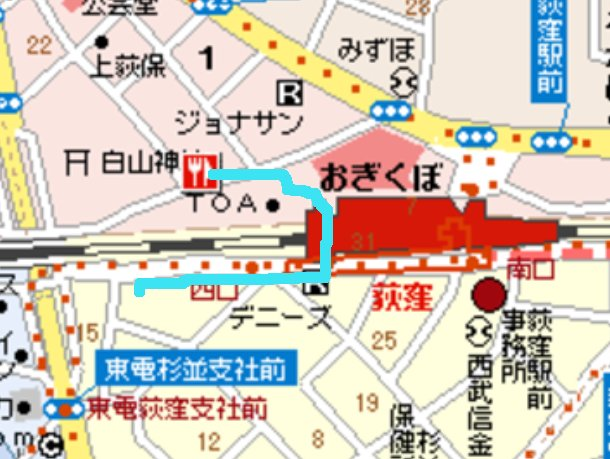
\includegraphics[width=0.5\hsize]{image200804/enkaimap.jpg}
\end{center}

\begin{itemize}
 \item 宴会場所\\
       本日の宴会は「駒忠」です。\\
       参加者はB1Fに集合し、全員で移動しましょう。
 \item 片付け\\
       部屋を片付けるのにご協力ください。
\end{itemize}

\end{frame}

\end{document}

;;; Local Variables: ***
;;; outline-regexp: "\\([ 	]*\\\\\\(documentstyle\\|documentclass\\|emtext\\|section\\|begin{frame}\\)\\*?[ 	]*[[{]\\|[]+\\)" ***
;;; End: ***
